\documentclass[11pt]{scrartcl}
\usepackage[utf8]{inputenc}
\usepackage{evank}


%% insert title here
\newcommand{\titlee}{Thermo I}
\parindent 0 pt

\newcommand{\officialsol}[1]{See the official solutions \href{#1}{here}.}

\title{\titlee}
\author{Cambridge Physics Academy}
\date{2023-2024}


\begin{document}

\thispagestyle{empty}
\begin{center}
    
    
    \Huge \textbf{\textsf{\titlee}}

    \large \theauthor
\end{center}

\setcounter{section}{-1}
\section{Readings}
\begin{itemize}
    \item Ch 21 and 23 of HRK
\end{itemize}
Feel free to do problems from the readings as extra practice.


\section{Lecture review}

\begin{defn}[Temperature and Heat]
    Temperature and heat are related by the heat capacitance of an object: $$\Delta Q=C\Delta T$$ The heat capacitance of some material can sometimes be measured per unit mass or per mole. 
\end{defn}

\begin{theorem}[Thermal Expansion]
    When an object is heated, each of its dimensions expand according to $$\Delta L=\alpha L\Delta T,$$ where $\alpha$ is a constant with $\alpha \ll 1$. Consequently, area and volume scale approximately as $$\Delta A=2\alpha A\Delta T\qquad \Delta V=3\alpha V\Delta T$$
\end{theorem}

\begin{defn}[First Law of Thermodynamics]
    The First Law is conservation of energy. If heat $\Delta Q$ is inputted into a system, the heat becomes $\Delta E$ of internal energy and $\Delta W$ of work done by the system on its surroundings: $$\Delta Q=\Delta E+\Delta W$$
\end{defn}

\begin{defn}[Ideal Gas Law]
    An ideal gas is an approximation for a real gas by ignoring the interactions between molecules of the gas (electrostatic, polarization, chemical reactions). An ideal gas follows the ideal gas law, which can be written in two forms: $$PV=nRT\qquad PV=Nk_BT$$ where $R=8.31\, \unit{J/mol\cdot K}$ is the ideal gas constant and $k_B=1.38\times 10^{-23}\, \unit{J/K}$ is the Boltzmann constant. 
\end{defn}

\begin{defn}[Internal Energy of Ideal Gas]
    We characterize the molecules of an ideal gas with its degrees of freedom $f$. A monatomic molecule has $f=3$, a diatomic molecule has $f=5$, and a polyatomic molecule has $f=6$. The constant volume molar heat capacity of an ideal gas is $$c_V=\frac{f}{2}R$$The internal energy of an ideal gas is $$E=nc_VT$$
\end{defn}

\begin{defn}[Adiabatic Constant]
    The constant pressure molar heat capacity of an ideal gas is $$c_P=\frac{f+2}{2}R$$The adiabatic constant $\gamma$ of the gas is then defined as $$\gamma=\frac{c_P}{c_V}=\frac{f+2}{f}$$
\end{defn}

\begin{theorem}[Adiabatic Processes]
    An adiabatic process is that in which there is no heat transfer into a gas, i.e. $\Delta Q=0$. Under these conditions, $$PV^\gamma=\text{const}$$and the work done by the gas can be shown to be $$W=\frac{1}{1-\gamma}(P_fV_f-P_0V_0)$$
\end{theorem}

\section{Problem Set}

\subsection{Exercises}



\begin{prob}[HRK]
    Dumet wire was developed to allow for the expansion of glass in lightbulbs. The wire consists of a core of nickel–steel with expansion coefficient $\alpha_n$ surrounded by a sheath of copper with expansion coefficient $\alpha_c$. The diameters of the core and of the sheath are chosen so that the wire duplicate the expansion characteristics of glass, which has coefficient $\alpha_g$. Show that the ratio of the nickel–steel radius to that of the copper sheath should be $$\frac{r_n}{r_c}=\sqrt{\frac{\alpha_c-\alpha_g}{\alpha_c-\alpha_n}}$$
\end{prob}

\begin{sol}
    We want $$\alpha_nr_n^2+(r_c^2-r_n^2)\alpha_c=\alpha_gr_c^2\Rightarrow \frac{r_n}{r_c}=\boxed{\sqrt{\frac{\alpha_c-\alpha_g}{\alpha_c-\alpha_n}}}$$
\end{sol}

\begin{prob}
    Two thermally insulated and isolated chambers each originally contain gasses with parameters $P_1,V_1,T_1$ and $P_2,V_2,T_2$. The chambers are then connected by a tube. Find the final pressure $P$ and temperature $T$ in the gas. 
\end{prob}

\begin{sol}
    Notice that the total internal energy in each chamber is proportional to $PV$ by the ideal gas law. Since the total energy is conserved, $$P_1V_1+P_2V_2=P(V_1+V_2)\Rightarrow P=\boxed{\frac{P_1V_1+P_2V_2}{V_1+V_2}}$$ There are $n=(P_1V_1/RT_1)+(P_2V_2/RT_2)$ total moles, so $$T=\frac{P(V_1+V_2)}{nR}=\boxed{\frac{(P_1V_1+P_2V_2)T_1T_2}{P_1V_1T_2+P_2V_2T_1}}$$
\end{sol}

\begin{prob}
    A vessel of volume $V$ containing one mole of diatomic gas at pressure $P$ is initially split in half by a thermally insulating piston. 
    \begin{anum}
        \item Some amount of heat $Q$ is given to the gas in one half of the vessel while the piston is held fixed. Then, the piston is released. Find the ratio of the volume of the heated to unheated half after the system reaches equilibrium. 
        \item A hole suddenly opens up in the piston, which allows gas to pass through both sides. After a long time, find the ratio of the volumes of the halves. 
        \item Find the final temperature $T$ of the gas. 
    \end{anum}
\end{prob}

\begin{sol}
    \begin{anum}
        \item Note that $Q=nc_V\Delta T=(5/2)\Delta P(V/2)$, so the pressure on one half after heating becomes $$P'=P+\frac{4Q}{5V}$$ The internal energy of either side will stay constant afterward, so $PV$ will be a constant. We seek the volumes such that the pressure is equalized on both sides. Let the final volume of the unheated part be $V'$. Then, $$\frac{P'(V/2)}{V-V'}=\frac{P(V/2)}{V'}\Rightarrow V'=\frac{PV}{2P+(4Q/5V)}$$And so the ratio is $$\frac{V-V'}{V}=\boxed{\frac{P+(4Q/5V)}{2P+(4Q/5V)}}$$
        \item The pressure on both sides of the piston will always be $P$, so the piston will not feel any external force. Thus, we take the same answer from part (a).
        \item The initial temperature is $T_0=PV/R$, and the increase in temperature is given by $\Delta T=Q/(5/2)R$. Thus the final temperature is $$T=\boxed{\frac{PV}{R}+\frac{2Q}{5R}}$$
    \end{anum}
\end{sol}

\begin{prob}
    An empty graduated cylinder of length $L$ and base area $A$ is oriented with its axis horizontal and spun in a circle about its open end at an angular speed $\omega$. The atmospheric pressure is $P_0$, the atmospheric temperature is $T_0$, and the molar mass of the atmosphere is $\mu$. Assume the gas in the cylinder is always at temperature $T_0$. 
    \begin{anum}
        \item Find the pressure $P$ at the closed end of the cylinder. 
        \item Set up, but do not evaluate, an integral for the total mass of the gas in the cylinder. 
    \end{anum}
\end{prob}

\begin{sol}
    \begin{anum}
        \item Using force balance on a small parcel of air a distance $r$ from the pivot, $$dP \, A=\rho A\omega^2r\, dr$$By the ideal gas law, $\rho=P\mu/RT_0$, so we get $$\int_{P_0}^P\frac{dP}{P}=\frac{\mu\omega^2}{RT_0}\int_0^Lr\, dr\Rightarrow P=\boxed{P_0e^{{\mu\omega^2L^2}/{2RT_0}}}$$
        \item At a distance $r$ from the pivot, the density is given by $\rho=(P_0\mu/RT_0)e^{{\mu\omega^2r^2}/{2RT_0}}$ from the previous part. Integrating this along the entire tube, $$m=\int_0^L\rho A\, dr=\boxed{\frac{P_0\mu A}{RT_0}\int_0^Le^{{\mu\omega^2r^2}/{2RT_0}} \, dr}$$
    \end{anum}
\end{sol}

\begin{prob}
    A piston of mass $m$ seals the top of a cylindrical chamber of base area $A$. The piston is initially a distance $h$ above the bottom of the chamber. The atmospheric pressure is $P_0$, and the atmosphere is diatomic.
    \begin{anum}
        \item What is the necessary pressure inside the chamber so that if the piston is released, it will not fall?
        \item Now assume the initial pressure in the chamber is $P_0$. The piston is released from rest. What is the final height of the piston above the bottom of the chamber? Assume there is no heat transfer between the gas in the chamber and its surroundings.
    \end{anum}
\end{prob}

\begin{sol}
    \begin{anum}
        \item By force balance, $$P=\boxed{P_0+\frac{mg}{A}}$$
        \item Let $h$ be the final height. Then, the work done by gravity is $mg(h-h')$, and the work done by the atmosphere is $P_0A(h-h')$. The internal energy of the gas at any point is equal to $(5/2)PV$ since the gas is diatomic. As a result, it holds that $$\frac 52P_0Ah+(mg+P_0A)(h-h')=\frac 52\left(P_0+\frac{mg}{A}\right)Ah'\Rightarrow h'=\boxed{\frac{7P_0A+mg}{7P_0A+2mg}h}$$
    \end{anum}
\end{sol}

\begin{prob}[IZhO]
    A quasistatic (slow, always in thermal equilibrium) process is carried out with one mole of an ideal monatomic gas, as a result of which its initial volume $V_0 = 1 \, \unit{m^3}$ increases four times, and the initial pressure $P_0 = 105 \, \unit{Pa}$ decreases two times. For each small section of the quasistatic process, the ratio of work to the change in internal energy is the same. Find the total work done by the gas in this process. 
\end{prob}

\begin{sol}
    The internal energy is given by $(3/2)RT=(3/2)PV$, since the gas is monatomic. Let the ratio of work to the change in internal energy be $\alpha$. Then, we are given that $$\frac32\alpha(P\, dV+V\, dP)=P\, dV\Rightarrow \left(1-\frac32\alpha\right)\frac{dV}{V}=\frac32\alpha\frac{dP}{P}$$ Integrating, we get $$\left(1-\frac32\alpha\right)\int_{V_0}^{4V_0}\frac{dV}{V}=\frac32\alpha\int_{P_0}^{P_0/2}\frac{dP}{P}\Rightarrow \left(1-\frac32\alpha\right)\ln 4=\frac32\alpha\ln \frac12\Rightarrow \alpha=\frac43$$The total work is thus $$W=\alpha\Delta E=\frac32\alpha \Delta (PV)=2P_0V_0=\boxed{2\times 10^5\, \unit{J}}$$
\end{sol}

\begin{prob}[CP]
    A thermally insulated cylinder with a movable, massless piston is connected to a thermally insulated tire of constant volume $V$ via a thermally insulated tube. During each pumping cycle, the valve in the tube is first closed. Then, the piston is expanded until the pressure and volume of the gas becomes $P_a$ and $V_a$, by taking air in from outside. The gas in the piston, which has an adiabatic index $\gamma$, is then compressed adiabatically until its volume becomes $V_a/2$. Finally, the valve is opened until equilibrium is reached between the container and the tire. If the tire does not contain any gas initially, determine the minimum number of cycles required to increase the pressure in the tire to $2^{\gamma-1}P_a$. 
    \begin{center}
        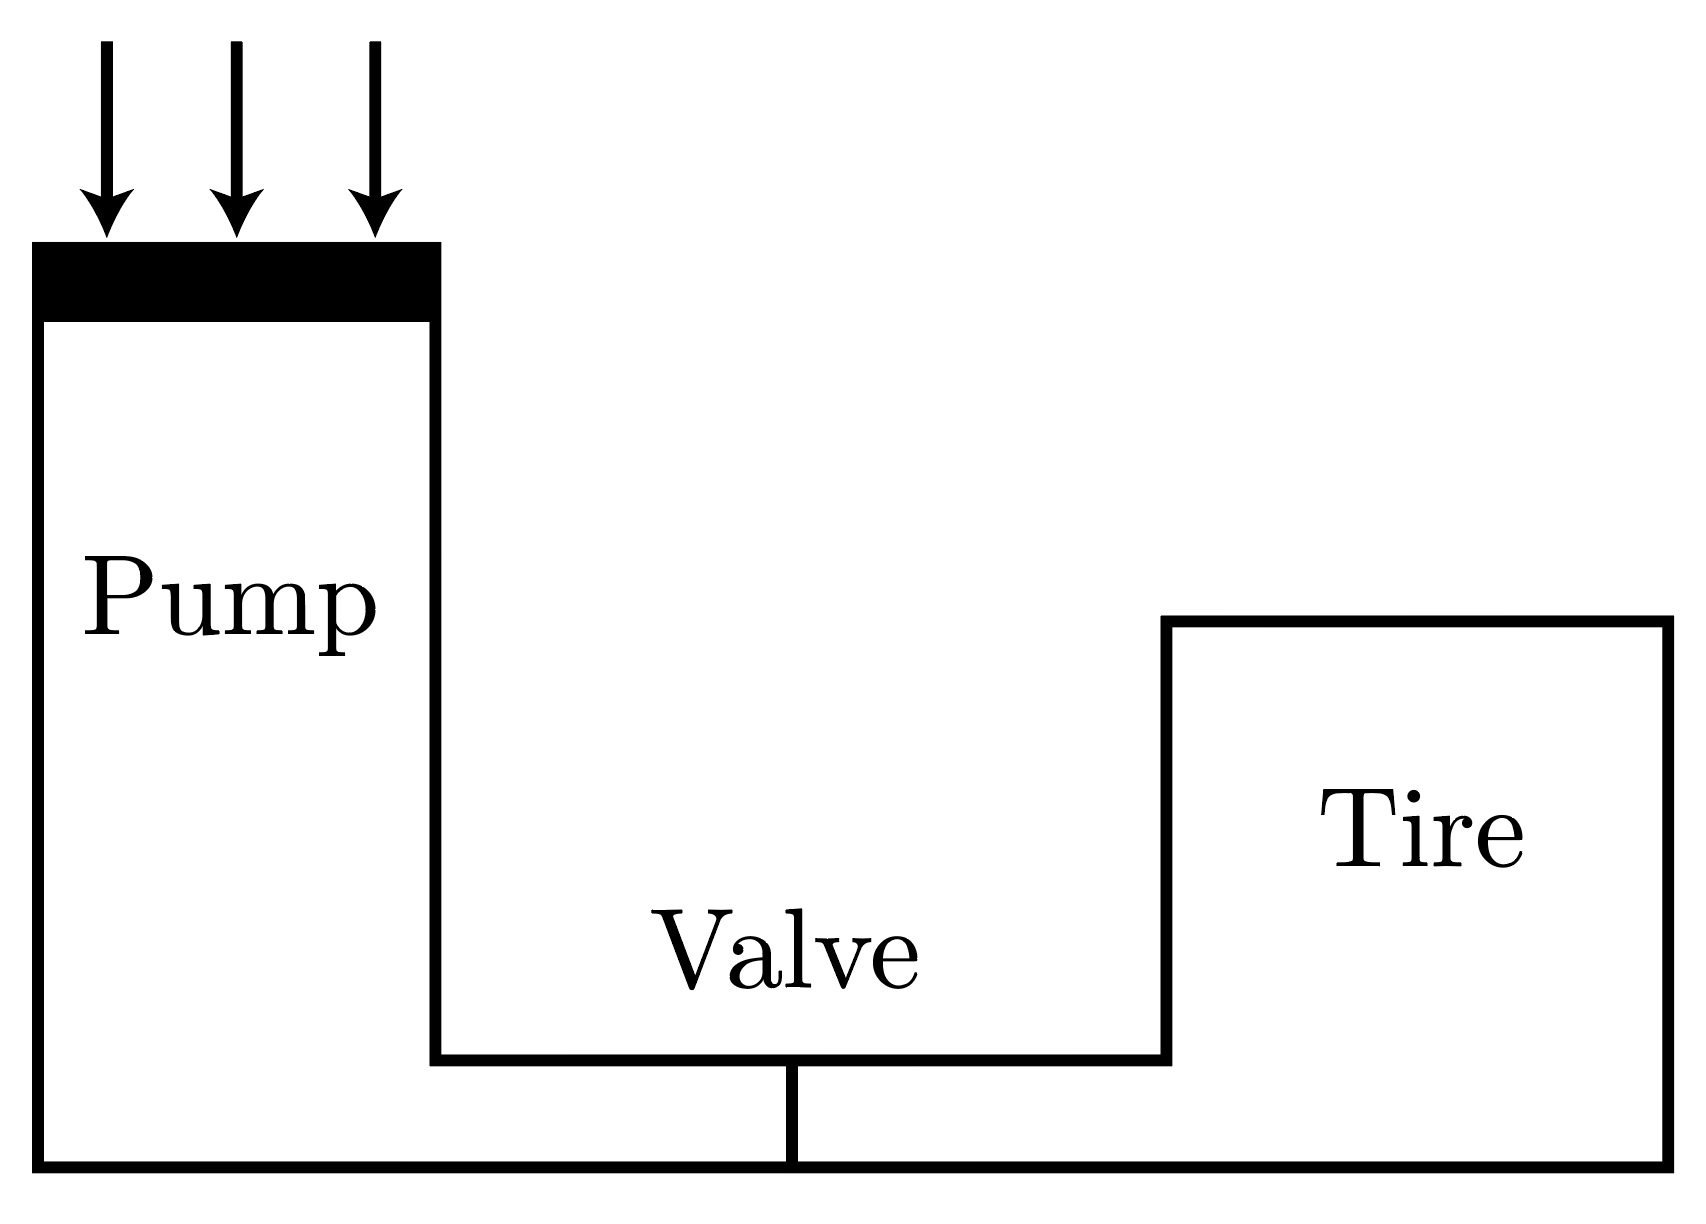
\includegraphics[scale=0.2]{cp1}
    \end{center}
\end{prob}

\begin{sol}
    Let the pressure of the gas after the adiabatic compression be $P_a'$. Then by the adiabatic condition, $$P_aV_a^\gamma=P_a'\left(\frac{V_a}{2}\right)^\gamma\Rightarrow P_a'=2^\gamma P_a$$Now, let the pressure in the tire after the $i$th cycle be $P_i$. When the gas in the pump and the existing gas in the tire mix, their total internal energy stays the same, so that the final pressure after mixing is found via $$P_{i+1}=\frac{P_iV+P_a'(V_a/2)}{V+(V_a/2)}=\frac{2^\gamma P_aV_a+2p_iV}{V_a+2V}$$Rearranging, we get $$P_{i+1}-2^\gamma P_a=\frac{2V}{V_a+2V}(P_i-2^\gamma P_a)$$This follows the form of a geometric progression with $P_0=0$, so $$P_n-2^\gamma P_a=\left(\frac{2V}{V_a+2V}\right)^n(-2^\gamma P_a)$$ Setting $P_n=2^{\gamma-1}P_a$, we get $$\left(\frac{2V}{V_a+2V}\right)^n=\frac12\Rightarrow n=\boxed{-\left(\log_2\frac{2V}{V_a+2V}\right)^{-1}}$$
\end{sol}

\begin{prob}[APhO]
Consider $n=2$ moles of ideal monatomic gas at a pressure $P_0$, volume $V_0$ and temperature $T_0= 300 \, \unit K$ placed in a vertical cylindrical container. A movable frictionless horizontal piston of mass $m = 10 \, \unit{kg}$ (assume $g = 9.8 \, \unit{m/s^2}$) and cross section $A= 500 \, \unit{cm^2}$ compresses the gas leaving the upper section of the container void. There is a vertical spring attached to the piston and the upper wall of the container. Let the spring constant $k=mgA/V_0$. Disregard any gas leakage through their surface contact, and neglect the specific thermal capacities of the container, piston and spring. Initially the system is in equilibrium and the spring is unstretched. Neglect the spring’s mass. Assume all processes within the gas are adiabatic.
\begin{center}
    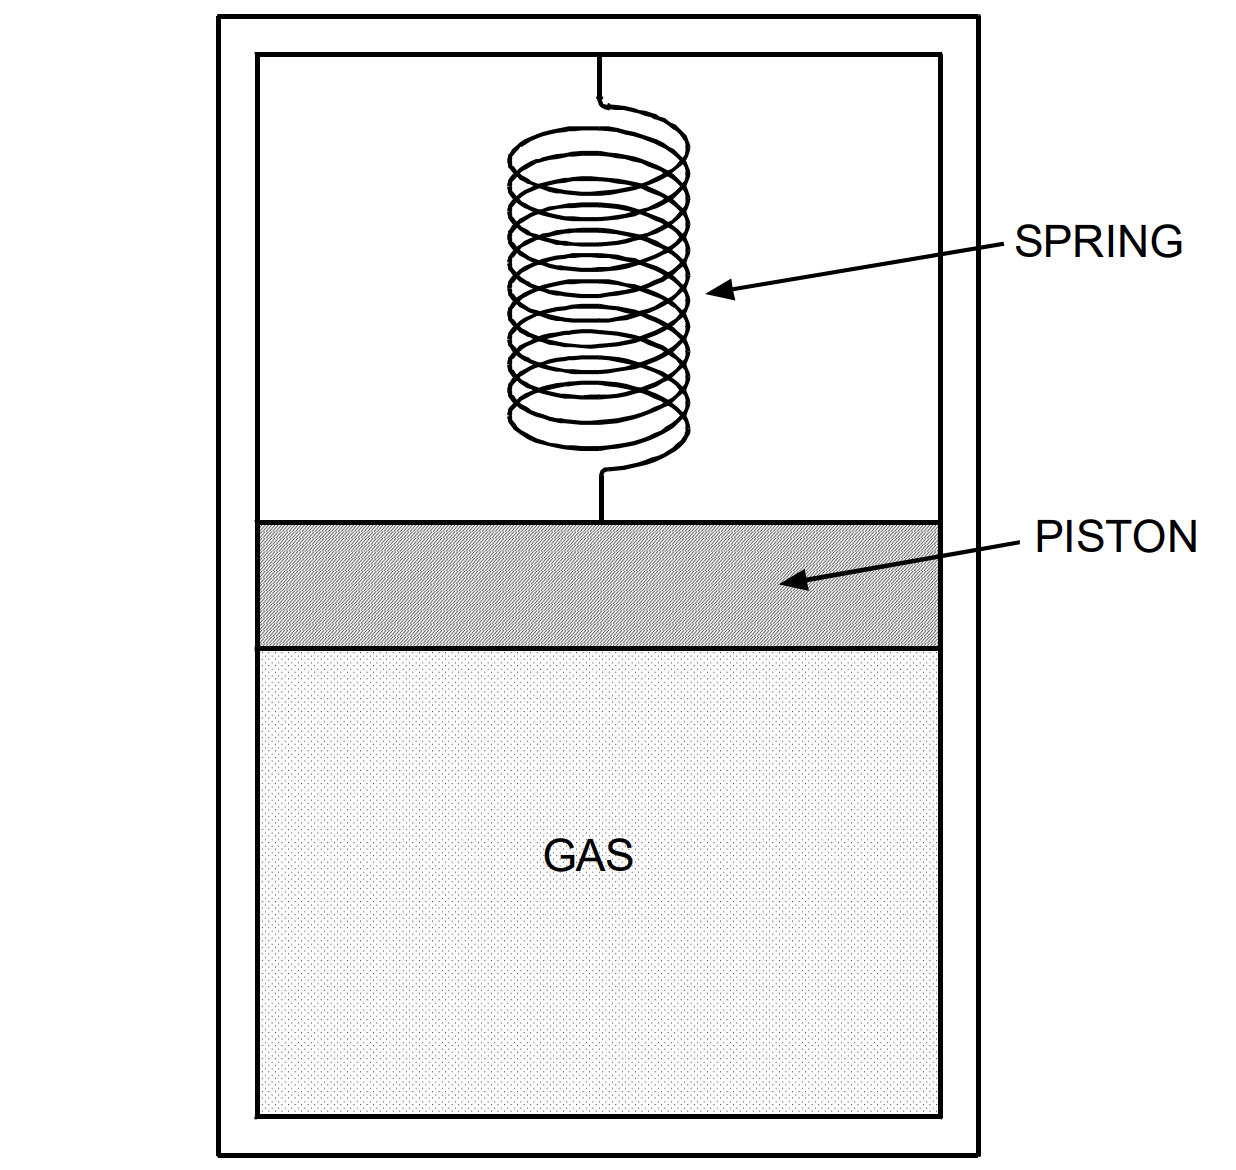
\includegraphics[scale=0.25]{piston}
\end{center}
\begin{anum}
    \item Calculate the frequency $f$ of small oscillations of the piston, when it is slightly displaced from equilibrium position. 
    \item Then the piston is pushed down until the gas volume is halved, and released with zero velocity. Calculate the value(s) of the gas volume when the piston speed is $$v=\sqrt{\frac{4gV_0}{5A}}$$
\end{anum}
\end{prob}

\begin{sol}
    See solutions \href{https://apho.olimpicos.net/pdf/APhO_2005_S1.pdf}{here} (Problem 1A). 
\end{sol}

\begin{prob}
    An atmosphere filled with a diatomic gas of pressure $P_0$ and temperature $T_0$ surrounds a chamber of volume $V$. A hole is created in the chamber and gas flows in. Assume the chamber is insulated so no heat is transferred through its walls. 
    \begin{anum}
        \item Let a small piece of air $dV$ enter the chamber. What is the internal energy of this small piece of air?
        \item What is the work done by external pressure on this piece of air as it moves into the chamber?
        \item What is the final temperature of the air in the chamber after airflow stops?
    \end{anum}
\end{prob}

\begin{sol}
    \begin{anum}
        \item The air is diatomic, so the internal energy is $$dE=\frac52nRT_0=\boxed{\frac52P_0\, dV}$$
        \item The work done by external pressure is $$dW=\boxed{P_0\, dV}$$
        \item The total energy of the gas in the chamber includes its initial internal energy and the external work done on the gas (by Newton's third law, the work done on $dV$ from the gas existing in the chamber is the negative of the work that $dV$ does on the gas in the chamber, so macroscopically this component cancels out). Thus, $$T_f=\frac{E_f}{(5/2)nR}=\frac{(5/2)P_0V+P_0V}{(5/2)nR}=\frac{(7/2)nRT_0}{(5/2)nR}=\boxed{\frac75T_0}$$
    \end{anum}
\end{sol}

\begin{prob}
    Using the definition $W=\int P\, dV$, derive the work done by a gas during an adiabatic process: $$W=\frac{1}{1-\gamma}(P_fV_f-P_0V_0)$$
\end{prob}

\begin{sol}
    Since $PV^\gamma=\text{const}$, we have $$W=\int_{V_0}^{V_f} P\, dV=P_0V_0^\gamma\int_{V_0}^{V_f} V^{-\gamma}\, dV=\frac{1}{1-\gamma}(P_0V_0^\gamma V_f^{1-\gamma}-P_0V_0)$$Note that since $P_f=P_0V_0^\gamma V_f^{-\gamma}$, substituting this in yields the desired $$W=\boxed{\frac{1}{1-\gamma}(P_fV_f-P_0V_0)}$$
\end{sol}

\begin{prob}[EstPhO]
    There is wet wood burning in a fireplace on the ground. Seven meters above ground, the smoke is at a temperature of $t_7 = 40^\circ \,\unit C$. Disregard the exchange of heat with the surrounding air and assume that the atmospheric pressure at the ground is constant in time and equal to $p_0 = 1\times 10^5\, \unit{Pa}$; the air temperature $t_0 = 20^\circ\, \unit{C}$ is independent of height. Assume that the smoke represents an ideal gas of a molar mass $\mu = 29 \,\unit{g/mol}$ (i.e. equal to the molar mass of the air), and of a molar specific heat at constant volume $c_V = 2.5R$; universal gas constant $R = 8.31 \, \unit{J/kg\cdot K}$. How high will the smoke column rise?
\end{prob}

\begin{sol}
    See solutions \href{https://www.ioc.ee/~kalda/ipho/es/e-s-08-sol.pdf}{here} (Problem 7).
\end{sol}

\begin{prob}
    The efficiency $\epsilon$ of a thermodynamic process is defined as the total work done by a gas in the process divided by the total heat input into the gas: $\epsilon =W/Q_{\text{in}}$. In this problem we analyze the efficiencies of different processes. In all $PV$ diagrams below, the gas moves in a clockwise path so that the work done is positive. Assume the gas is diatomic.
    \begin{anum}
        \item Find the efficiency of the cycle below in terms of $P_1,P_2,V_1,V_2$. 
        \begin{center}
            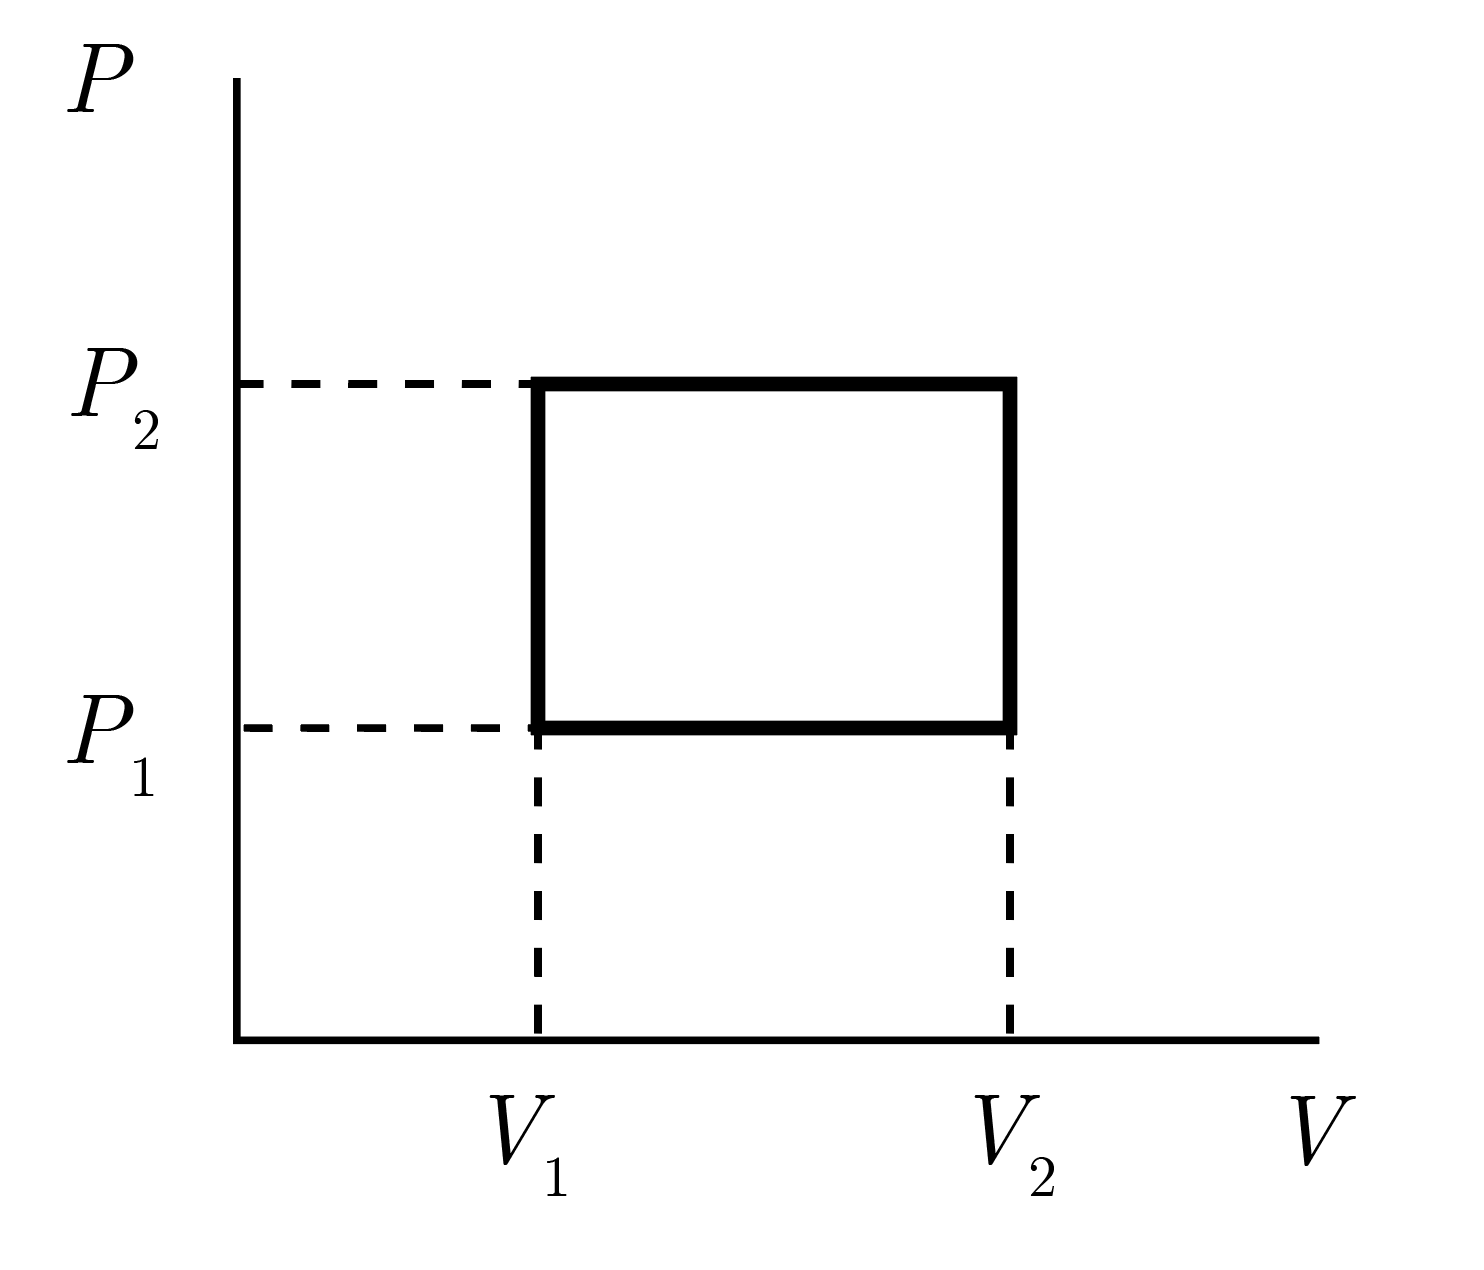
\includegraphics[scale=0.2]{gr1}
        \end{center}
        \item Find the efficiency of the cycle below in terms of $P_1,P_2,V_1,V_2$.
        \begin{center}
            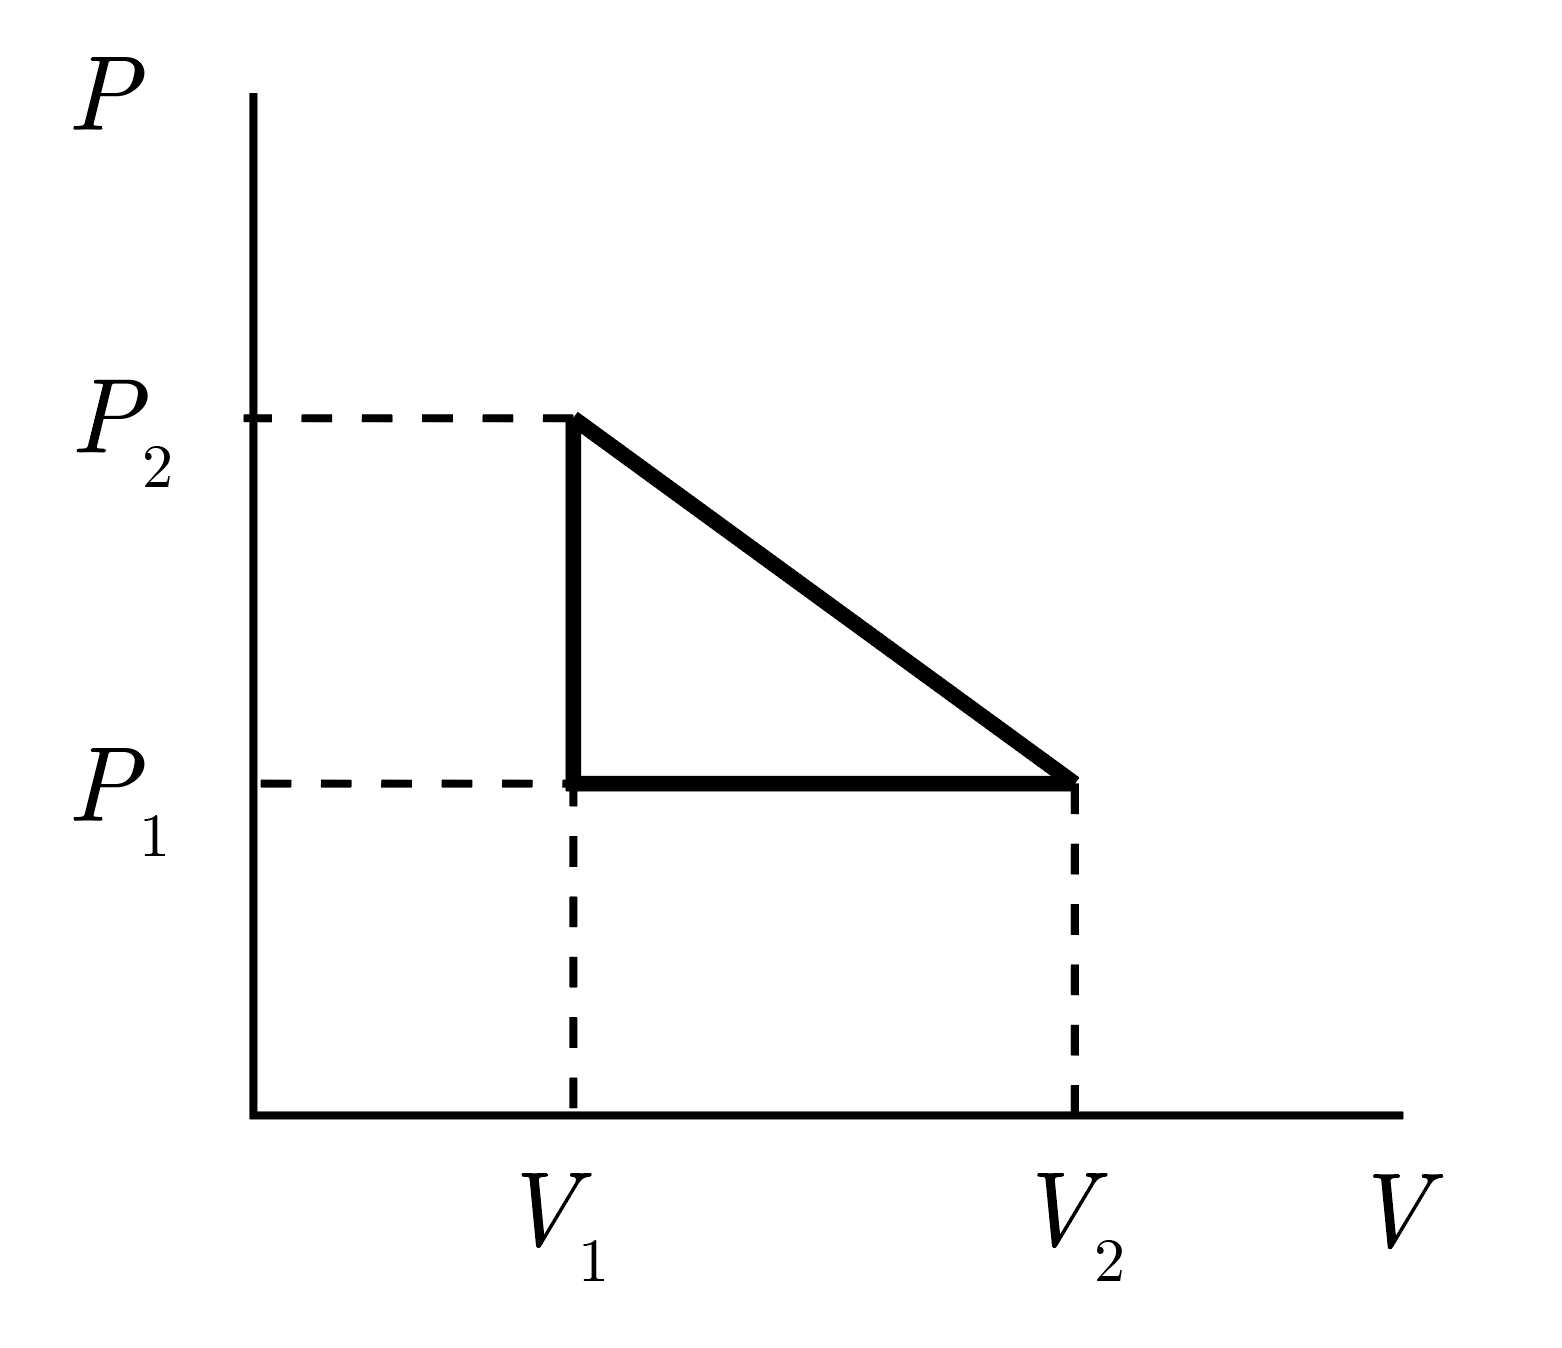
\includegraphics[scale=0.2]{gr2}
        \end{center}
        \item The cycle below has two isotherms bounded by adiabats. Find the efficiency of the cycle below in terms of $T_1,T_2$. This is a special cycle called the Carnot cycle. 
        \begin{center}
            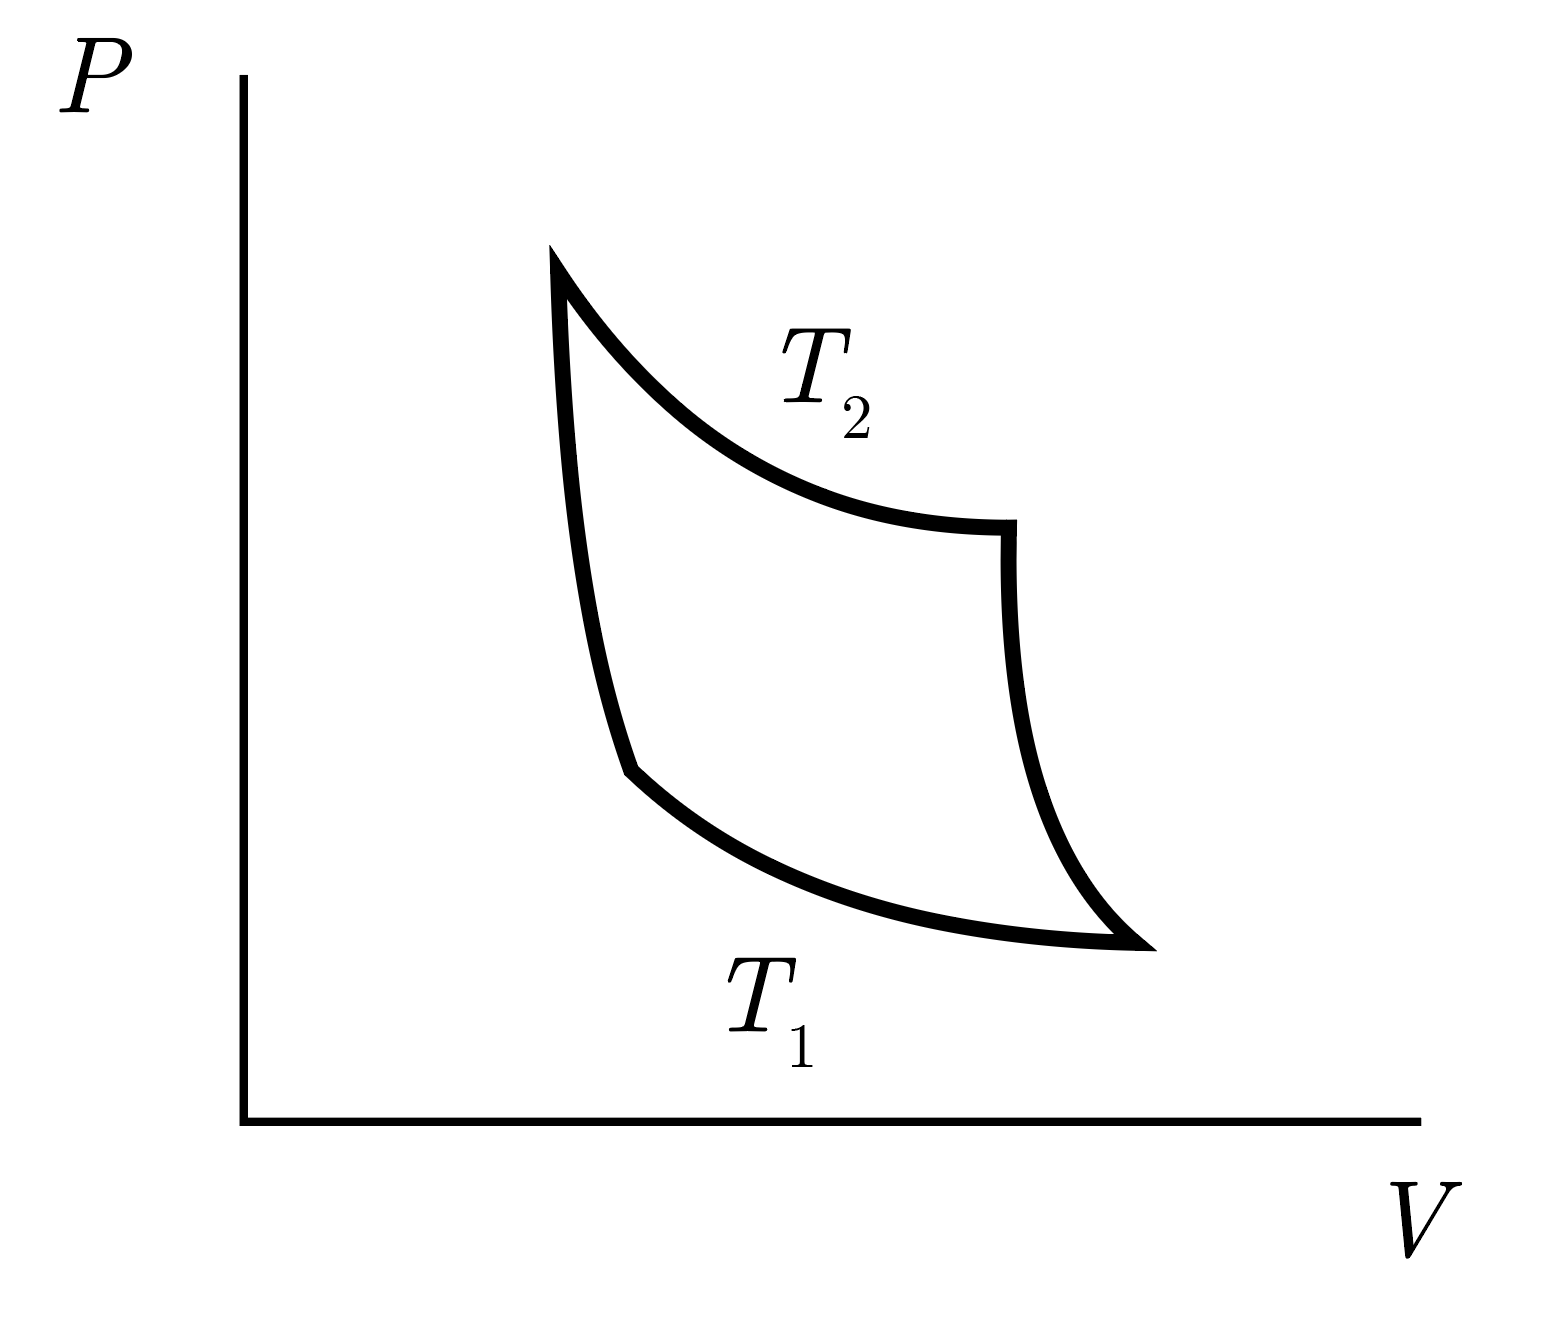
\includegraphics[scale=0.2]{gr4}
        \end{center}
    \end{anum}
\end{prob}

\begin{sol}
    \begin{anum}
        \item The heat input is done on the left and top sides of the rectangle, and here we can use $c_V$ and $c_P$. $$Q_{\text{in}}=\frac52V_1(P_2-P_1)+\frac72P_2(V_2-V_1)$$The total work done is the area of the rectangle. Thus, the efficiency is $$\epsilon=\boxed{\frac{(P_2-P_1)(V_2-V_1)}{(5/2)V_1(P_2-P_1)+(7/2)P_2(V_2-V_1)}}$$
        \item The heat in on the left side is $(5/2)V_1(P_2-P_1)$, and the work done is the area of the triangle. The tricky part is finding the heat input along the diagonal. Analyzing the diagonal via the the first law of thermodynamics, we have $$\Delta Q=\Delta E+\Delta W=\frac52(P_1V_2-P_2V_1)+P_1(V_2-V_1)+\frac12(P_2-P_1)(V_2-V_1)$$Thus from summing up the total heat in, $$\epsilon = \frac{(P_2-P_1)(V_2-V_1)}{-6P_1V_1+6P_1V_2-P_2V_1+P_2V_2}=\boxed{\frac{P_2-P_1}{P_2+6P_1}}$$
        \item Note that because of the adiabatic invariant, the ratio of the volumes of the gas between each isotherm is the same. Let this ratio be $r$. The heat transfer into the system is only done on the $T_2$ isotherm, and this is equal to the work the gas does: $Q_{\text{in}}=nRT_2\ln r$. The total work done by the gas is $W=nR(T_2-T_1)\ln r$. Thus, the efficiency is $$\epsilon=\boxed{1-\frac{T_1}{T_2}}$$You will see next week that this is the maximum possible efficiency of an engine. 
    \end{anum}
\end{sol}

\subsection{Challenge Problems}

\begin{prob}[NBPhO]
    There are three beams between two absolutely rigid plates. The weight of the plates and the beams can be neglected. The coefficient of thermal expansion of the beams is $\alpha = 1.0\times 10^{-5}\, \unit{K^{-1}}$. The maximum strain (relative length change compared to the no load case) before permanent inelastic deformations of the material of the beam is $\beta = 0.40$\%. The beams can support a maximum amount of weight on the top plate, at which point permanent deformations start taking place in some of the beams.
    \begin{center}
        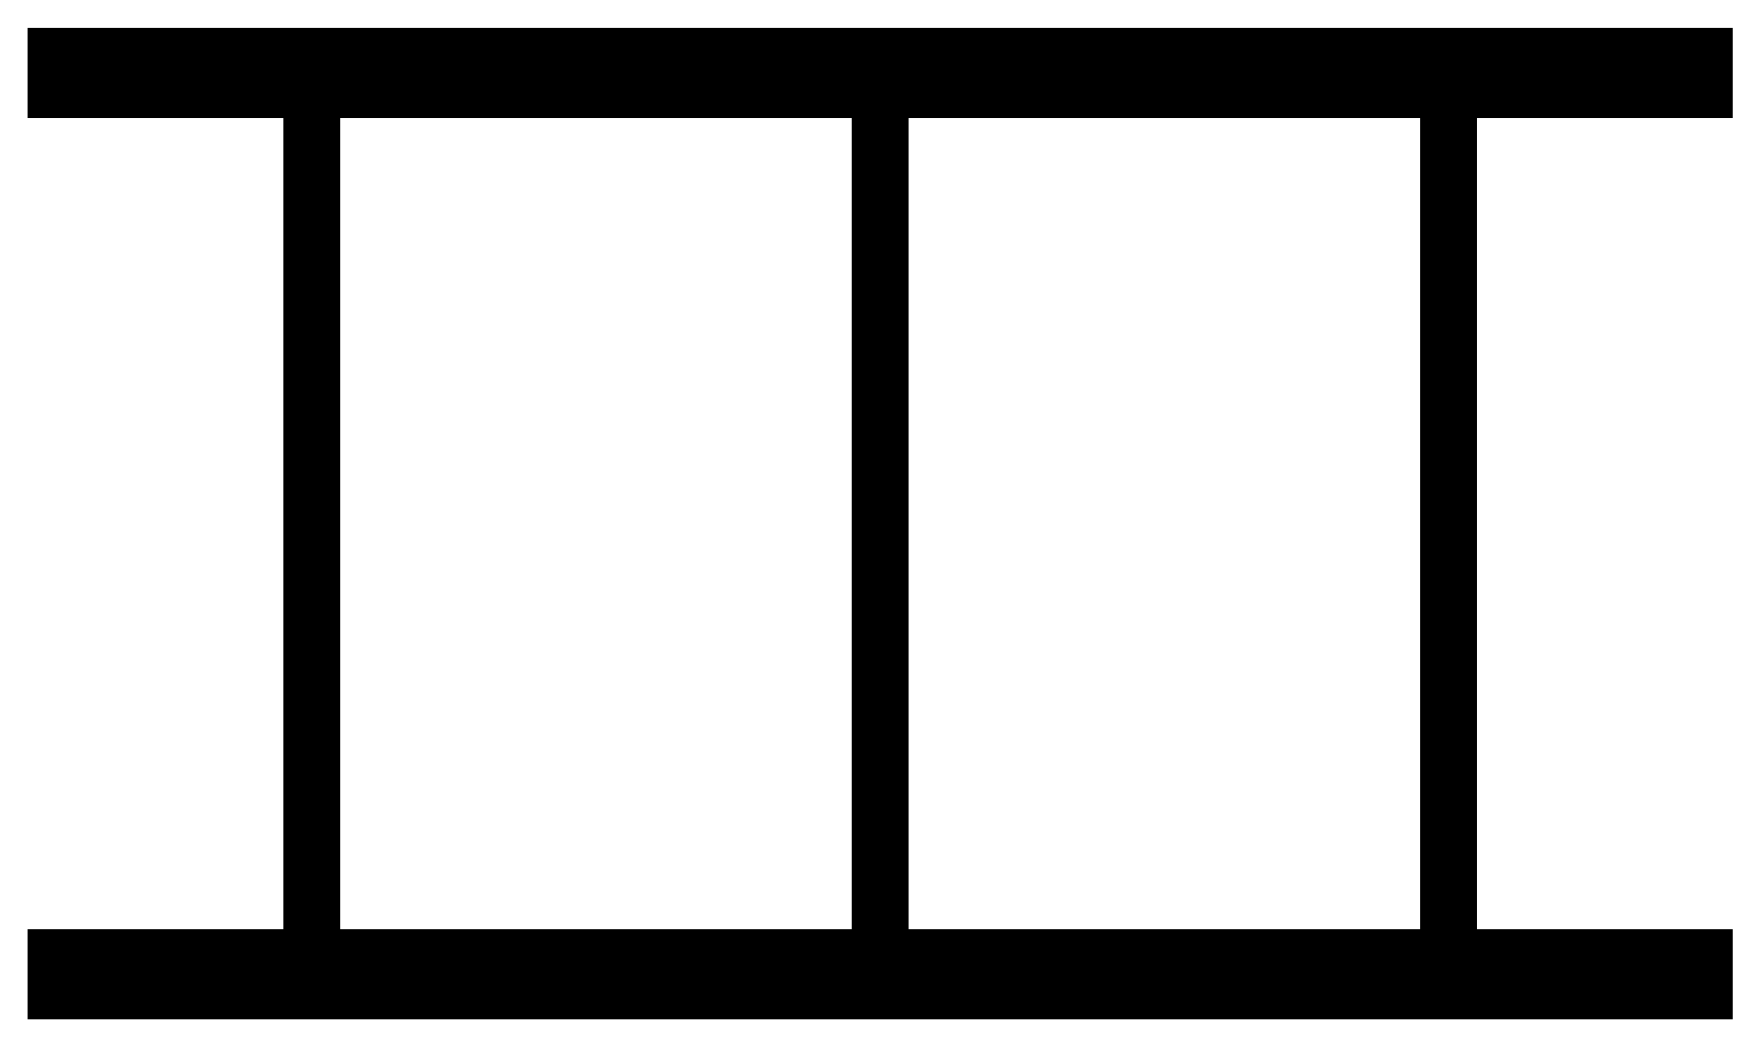
\includegraphics[scale=0.2]{grece}
    \end{center}
    \begin{anum}
    \item Initially all the beams are at the same temperature. Then the temperature of the beam in the middle is increased by $\Delta T = 100\, \unit{K}$. Compared to the case when the beams were at equal temperatures, what fraction of the original maximal weight can the beams now support on the top plate? Assume that the properties of the materials (specifically the maximum strain and the elastic modulus) don’t change during the heating.
    \item All of the beams are originally at temperature $T_0 = 0^\circ \, \unit{C}$. A load of 20\% of the maximal load is placed on the top plate. Keeping the same load on, to what temperature can the beam in the middle be heated such that no permanent deformations occur? This time the elastic modulus of the material changes depending on the temperature as shown in the figure below.
    \begin{center}
        
\includegraphics[scale=0.3]{graf}
    \end{center}
    \end{anum}
\end{prob}

\begin{sol}
    See solutions \href{https://www.ioc.ee/~kalda/ipho/es/NBPhO17_sol.pdf}{here} (Problem 8).
\end{sol}

\subsection{USAPhO Practice}

\begin{prob}[USAPhO 2018 A3]
    A vacuum system consists of a chamber of volume $V$ connected to a vacuum pump that is a cylinder with a piston that moves left and right. The minimum volume in the pump cylinder is $V_0$, and the maximum volume in the cylinder is $V_0 + \Delta V$. You should assume that $\Delta V\ll V$.
    \begin{center}
        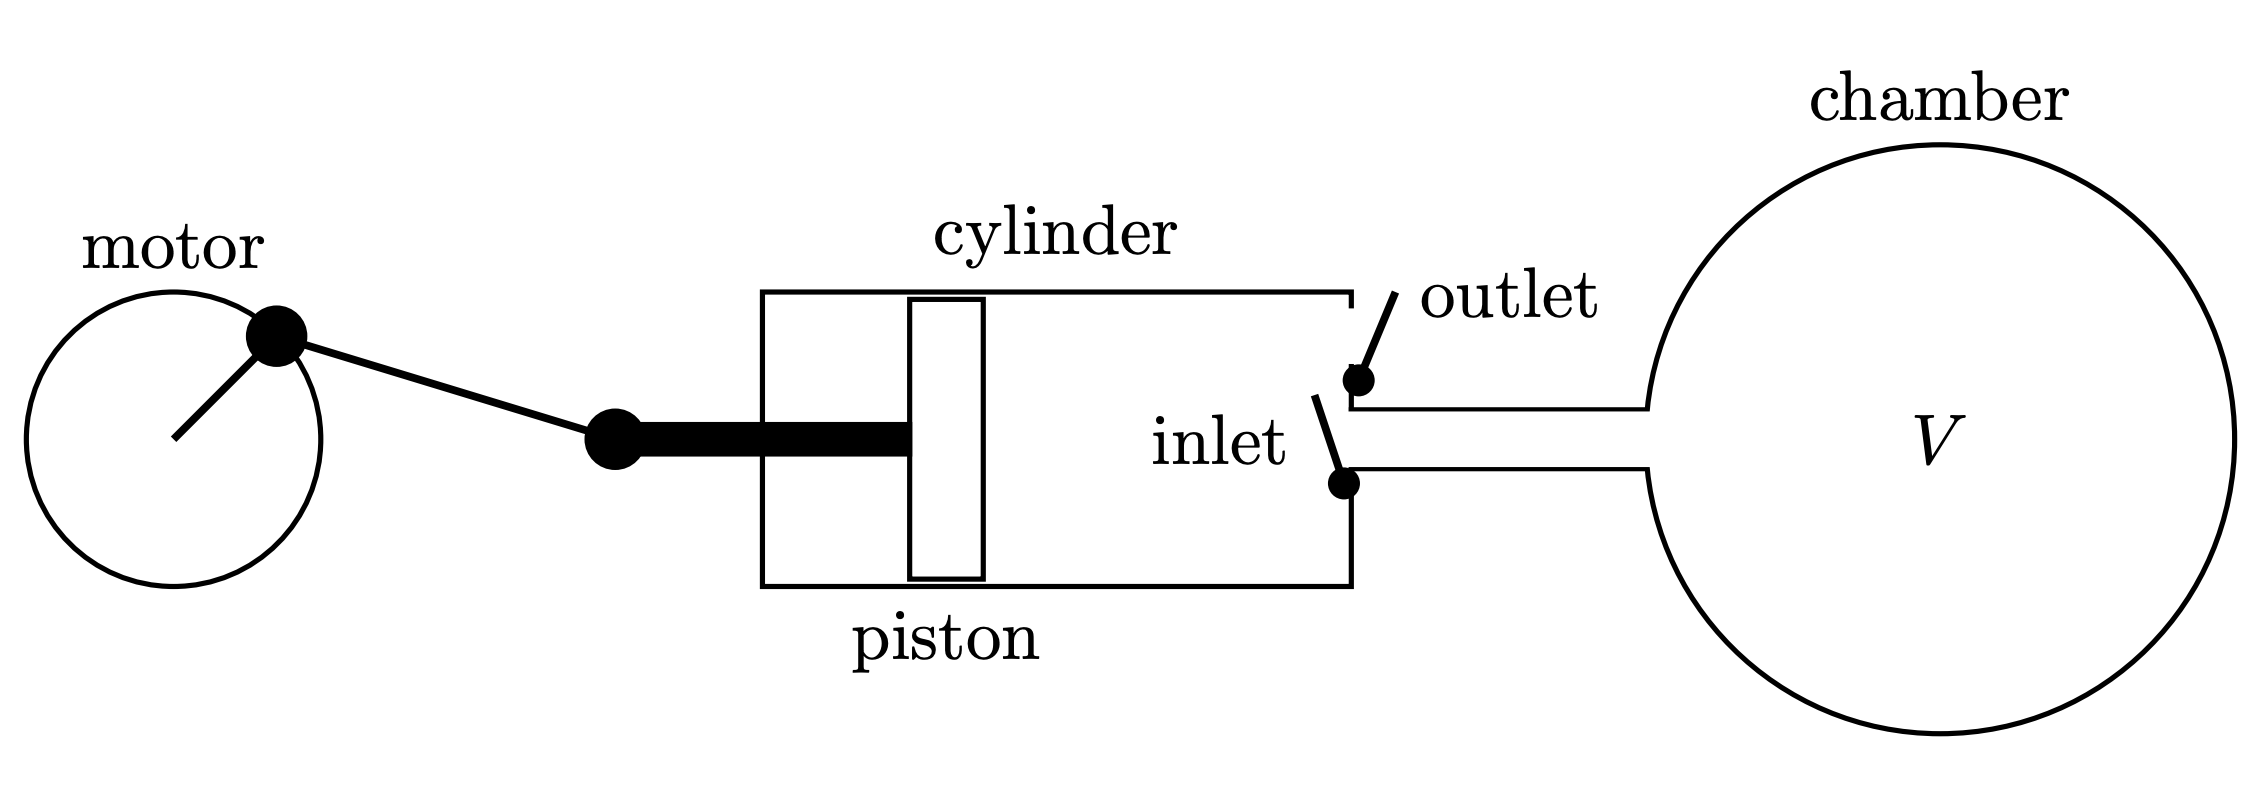
\includegraphics[scale=0.3]{motor}
    \end{center}
    The cylinder has two valves. The inlet valve opens when the pressure inside the cylinder is lower than the pressure in the chamber, but closes when the piston moves to the right. The outlet valve opens when the pressure inside the cylinder is greater than atmospheric pressure $P_a$, and closes when the piston moves to the left. A motor drives the piston to move back and forth. The piston moves at such a rate that heat is not conducted in or out of the gas contained in the cylinder during the pumping cycle. One complete cycle takes a time $\Delta t$. You should assume that $\Delta t$ is a very small quantity, but $\Delta V/\Delta t=R$ is finite. The gas in the chamber is ideal, monatomic, and remains at a fixed temperature of $T_a$. Start with assumption that $V_0 = 0$ and there are no leaks in the system.
    \begin{anum}
        \item At $t = 0$ the pressure inside the chamber is $P_a$. Find an equation for the pressure at a later time $t$.
        \item Find an expression for the temperature of the gas as it is emitted from the pump cylinder into the atmosphere. Your answer may depend on time.
        \item For this part, $0 < V_0 < \Delta V \ll V$. Find an expression for the minimum possible pressure in the chamber, $P_{\text{min}}$.
    \end{anum}
    
\end{prob}

\begin{sol}
    See solutions \href{https://aapt.org/physicsteam/2019/upload/USAPhO-2018-Solutions.pdf}{here}. 
\end{sol}

\begin{prob}
    An initially airtight chamber is shaped like a cylinder of length $L$ with two pistons of mass $m$ and radius $r$ sealing the open ends. Assume the cylinder is perfectly rigid and that all processes are reversible. There are locks along the cylinder wall that initially hold the pistons in place. 
    \begin{anum}
        \item Initially, the cylinder contains a vacuum and it is surrounded by an atmosphere with pressure $P_0$ and adiabatic constant $\gamma$. The locks are released and the pistons start moving toward each other. What are their velocities right before they collide? 
        \item Assuming the collision between the pistons is elastic, what is the period of one ``oscillation" of the system?
        \item Now, assume initially the cylinder contains gas from the atmosphere but at a much lower pressure $P\ll P_0$. Find the minimum separation between the pistons after they are released. 
        \item At what separation between the pistons during the process in part (c) is the velocity of the pistons the highest?
    \end{anum}
\end{prob}

\begin{sol}
    \begin{anum}
        \item The work done by the atmosphere on each piston is equal to $P_0\pi r^2L/2$, and this equals the kinetic energy of each piston. Thus, $$\frac12P_0\pi r^2L=\frac12mv^2\Rightarrow v=\boxed{\sqrt{\frac{P_0\pi r^2L}{m}}}$$
        \item When the pistons are at a distance $x$ from their starting position, their velocities are given as $v=\sqrt{{P_0\pi r^2x}/{m}}$ from the previous part. Substituting $v=dx/dt$ and integrating, the time it takes for the pistons to collide is simply $$\int_0^{L/2}\frac{dx}{\sqrt x}=\sqrt{\frac{P_0\pi r^2}{m}}\int_0^tdt\Rightarrow t=\sqrt{\frac{2mL}{P_0\pi r^2}}$$We double this to find the period: $$T=2t=\boxed{2\sqrt{\frac{2mL}{P_0\pi r^2}}}$$
        \item The compression is very fast, so we assume the process is adiabatic. At the minimum separation of the pistons, the pistons do not carry any energy, so all the energy must have been stored in the gas. Using the formula for work done on an adiabatic gas (and canceling out $\pi r^2$ everywhere), $$\frac{1}{\gamma-1}(P_fd-PL)=P_0L$$Note that $P_f=P(L/d)^\gamma$ by the adiabatic invariant, so \begin{align*}
            \frac{1}{\gamma-1}(PL^\gamma d^{1-\gamma}-PL)=P_0L\Rightarrow P\left(\frac{L^{\gamma-1}}{d^{\gamma-1}}-1\right)=(\gamma-1)P_0
        \end{align*}Since $L\gg d$ we can neglect the $-1$ term in the parenthesis on the left, so solving for $d$ yields $$d=\boxed{L\left(\frac{P}{P_0(\gamma-1)}\right)^{\frac{1}{\gamma-1}}}$$
        \item The pistons stop accelerating when the pressure inside the chamber exceeds $P_0$, so the moment we are looking for is when the pressure in the chamber is exactly $P_0$. Using the adiabatic invariant, $$P_0d^\gamma=PL^\gamma\Rightarrow d=\boxed{L\left(\frac{P}{P_0}\right)^{\frac 1\gamma}}$$
    \end{anum}
\end{sol}


\end{document}